% HALQA — EdNova GenAI Peer-Learning Companion — Phase 1 Technical Report
% Compile: tectonic main.tex  (or pdflatex)
\documentclass[10pt,twocolumn]{IEEEtran}
\usepackage[utf8]{inputenc}
\usepackage[T1]{fontenc}
\usepackage{graphicx}
\usepackage{amsmath}
\usepackage{booktabs}
\usepackage{enumitem}
\usepackage{url}
\usepackage{xcolor}
\usepackage[hidelinks]{hyperref}
\usepackage{tikz}
\usetikzlibrary{arrows.meta,positioning,fit,backgrounds,calc}

\setlist{nosep,leftmargin=1.2em}
\definecolor{acc}{HTML}{1B2A5E}
\definecolor{accg}{HTML}{6A3FB5}

\newcommand{\trip}[1]{\textcolor{accg}{\textbf{#1}}}

\begin{document}

\title{
\includegraphics[width=3.2cm]{logo.png}\\[10pt]
HALQA: A GenAI Peer-Learning Companion\\that Puts the Circle First\\[6pt]
{\normalsize\mdseries Phase~1 Technical Report --- IEEE WIE ACT 5.0}\\[2pt]
{\normalsize\mdseries EdNova GenAI Peer-Learning Companion Challenge}}

\author{\IEEEauthorblockN{HALQA Team (3 members)}
\IEEEauthorblockA{\textit{AI/Backend (NestJS + MongoDB)} \textbullet{} \textit{Frontend/UX (React PWA)} \textbullet{} \textit{Data/Eval/Business}\\
November 2026}}

\maketitle

\begin{abstract}
Peer learning works best when everyone teaches --- yet study groups usually collapse into one dominant voice, passive listeners, and uncritical acceptance of wrong answers. \textbf{HALQA} (Arabic for \emph{circle}) is a GenAI learning companion that orchestrates \emph{human-first} group sessions and steps in only when the circle needs help. Every question is first offered to peers for 45--60\,s; meanwhile the AI prepares a hidden answer that is released only at the window's end, verified by an \emph{Auditor} step that catches incorrect peer answers before they spread. A single diagnostic ("learning DNA") steers a \emph{documented model-routing policy}: a compact model handles classification, hints, and short scaffolding; a larger model is reserved, on explicit escalation, for multi-source synthesis and polished synthesis --- measured at an L-share of \textbf{13.3\%} of calls against a $<25\%$ target. Retrieval-augmented generation with mandatory citations grounds every answer; a four-level degradation state machine (queue, retry, compact-model fallback, offline pack) keeps the circle alive when capacity or the larger model is unavailable. The system is multilingual by design (Arabic, Tunisian Darija with Arabizi, French, English), is privacy-preserving at the schema level, and ships with an adoption path for universities, training centers, and self-learning communities.
\end{abstract}

\section{Problem and Objective}
Learning is more effective when learners explain concepts to each other, but peer-to-peer learning is rarely structured: one person dominates, timid learners do not ask ``simple'' questions, unclear explanations go unchallenged, and a single explanation style never fits everyone. These dynamics appear in universities, workshops, training programs, and self-learning groups alike.

The EdNova challenge asks how Generative AI can act as \emph{mediator, teammate, tutor, and facilitator} to make learning structured, inclusive, interactive, personalized, and effective. Our design position is deliberate: \trip{the AI must not replace the circle --- it must make the circle work}. We therefore:

\begin{itemize}
\item guarantee every learner a fair turn: questions first go to \emph{peers} inside a timed window, and only then are AI answers revealed (Circle-First, AI-Second);
\item protect the group from wrong peer answers with an AI verification step (Auditor) and fact-checked consensus polls;
\item personalize via a short upfront diagnostic (the \emph{learning-DNA passport}) that tunes level, hint eagerness, register, and language, including Tunisian Darija with code-switching;
\item scaffold rather than solve: a hint ladder (L1--L4) and Socratic questioning before any direct answer;
\item treat platform constraints (shared access, scarce larger-model quota, seconds-scale latency) as a \emph{first-class design budget}, not an incident.
\end{itemize}

\section{Proposed Solution}
HALQA is a progressive web app (React + Vite PWA) backed by a REST API (NestJS~11, TypeScript strict, MongoDB). The companion agent, \textbf{Nova}, performs six roles inside a session:

\begin{itemize}
\item \textbf{Circle-First Ask (CF-AS).} A learner posts a question; peers answer and vote during a 45--60\,s window. In parallel --- invisibly --- HALQA retrieves, caches, and prepares the AI \emph{Quick Take}; the larger model is queued only if escalation fires. At window end (or skip), peers' answers are verified by the Auditor, the user gets staged progress, and the session is credited.
\item \textbf{Learning DNA.} A 4-question diagnostic captures level, preferred learning style (visual / analogy / step-by-step / practice), language register, and hint eagerness --- the ``diagnostic step to identify the method that fits each person best'' required by the track.
\item \textbf{Hint ladder.} L1 nudge $\rightarrow$ L2 analogy $\rightarrow$ L3 worked start $\rightarrow$ L4 full solution. The passport decides how early the ladder starts.
\item \textbf{Whisper chain fix (Teach-to-learn).} A peer paraphrases a chain of ideas; Nova compares it against claim checklists and returns a \emph{drift map} (kept / lost / distorted / added) plus one repair round --- explicitly detecting confusion and incorrect explanations.
\item \textbf{Consensus \& quizzes.} Polls on contested claims, Quiz Battles (3 items) and quiz generation, gamified credits and streaks, an automatic revision \emph{capsule} at session end, and a facilitator \emph{board} with per-circle health.
\item \textbf{S-B-U health rings.} Per circle, \emph{Share} (participation balance), \emph{Build} (help quality), \emph{Understand} (verified agreement) are computed from telemetry; \texttt{needs\_human} flags when the AI should defer to a mentor.
\end{itemize}

\section{System Architecture}
\subsection{Overview}
The backend is a NestJS service of 25 domain modules over 15 Mongo collections. Pure logic (PII scrubbing, credits math, cache keys, bandit, Arabizi normalization) lives in a dependency-free \texttt{domain/} layer and is unit-tested in isolation. All provider knowledge is confined to one adapter.

\begin{figure}[t]
\centering
\resizebox{\columnwidth}{!}{%
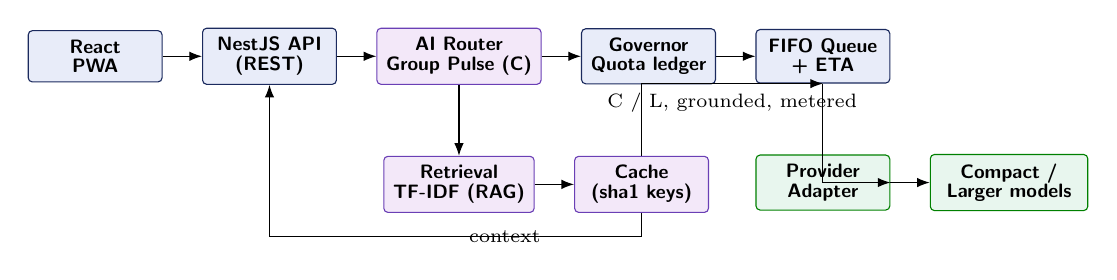
\begin{tikzpicture}[font=\scriptsize\bfseries\sffamily, node distance=4mm and 5mm, every node/.style={align=center}]
\definecolor{boxbg}{HTML}{E8ECF9}
\definecolor{rnbg}{HTML}{F3E8F9}
\definecolor{monbg}{HTML}{E8F6EE}
\tikzset{box/.style={draw=acc, fill=boxbg, rounded corners=1.5pt, minimum height=6mm, minimum width=17mm},
         mon/.style={draw=green!50!black, fill=monbg, rounded corners=1.5pt, minimum height=6mm, minimum width=17mm},
         rn/.style={draw=accg, fill=rnbg, rounded corners=1.5pt, minimum height=6mm, minimum width=17mm}}
\node[box] (pwa) {React\\[-1pt]PWA};
\node[box, right=of pwa] (nest) {NestJS API\\[-1pt](REST)};
\node[rn, right=of nest] (router) {AI Router\\[-1pt]Group Pulse (C)};
\node[box, right=of router] (gov) {Governor\\[-1pt]Quota ledger};
\node[box, right=of gov] (queue) {FIFO Queue\\[-1pt]+ ETA};
\node[mon, below=9mm of queue] (prov) {Provider\\[-1pt]Adapter};
\node[mon, right=of prov, minimum width=20mm] (models) {Compact /\\[-1pt]Larger models};
\node[rn, below=9mm of router] (ret) {Retrieval\\[-1pt]TF-IDF (RAG)};
\node[rn, right=of ret] (cache) {Cache\\[-1pt](sha1 keys)};
\draw[-{Latex[length=1.6mm]}] (pwa) -- (nest);
\draw[-{Latex[length=1.6mm]}] (nest) -- (router);
\draw[-{Latex[length=1.6mm]}] (router) -- (gov);
\draw[-{Latex[length=1.6mm]}] (gov) -- (queue);
\draw[-{Latex[length=1.6mm]}] (queue.south) |- (prov.east);
\draw[-{Latex[length=1.6mm]}] (prov) -- (models);
\draw[-{Latex[length=1.6mm]}] (router.south) -- (ret.north);
\draw[-{Latex[length=1.6mm]}] (ret) -- (cache);
\draw[-{Latex[length=1.6mm]}] (cache.north) |- node[pos=0.75, below, font=\scriptsize] {C / L, grounded, metered} (queue.south);
\draw[-{Latex[length=1.6mm]}] (cache.south) |- node[pos=0.75, left, font=\scriptsize] {context} ($(ret.south)+(0,-3mm)$) -| ($(nest.south)+(0,-3mm)$) -- (nest.south);
\end{tikzpicture}}%
\caption{Request path: every C/L call passes router $\rightarrow$ governor $\rightarrow$ queue $\rightarrow$ adapter, with retrieval-first grounding and a semantic cache in front; every hop is instrumented on \texttt{/metrics}.}
\end{figure}

\subsection{Two Model Categories --- a documented policy}
Inference runs without GPU acceleration and access is shared, so \emph{sending every request to the larger model to be safe} is a failure mode, and so is a ceiling imposed by the compact model alone. HALQA makes the split deliberate and measurable. A per-turn \emph{Group Pulse} routes intent (6-way), language/register, safety/PII, and the difficulty gate --- all compact-tier and batched into one schema-constrained call.

\begin{table}[t]
\caption{Model routing policy (Phase 1)}
\centering
\footnotesize
\begin{tabular}{@{}p{0.30\columnwidth}p{0.60\columnwidth}@{}}
\toprule
\textbf{Compact (C)} & \textbf{Larger (L) --- escalation only} \\
\midrule
Group Pulse routing; Quick Take drafts; hint ladder L1--L3; poll/quiz items; language rewriting; DNA interpretation; Whisper compare; mentor briefs & $\geq$3 retrieved chunks with conflict (multi-source synthesis); polished capsule/revision prose; low C confidence; explicit Whisper/Auditor escalation; deep-dive question \\
\bottomrule
\end{tabular}
\end{table}

The route targets live in configuration (\texttt{config/router.yaml}) and are verified by \texttt{/metrics}: skeleton $<200$\,ms, C-complete $<4$\,s, L-complete $<12$\,s, and \emph{L-share} $<25\%$ of calls. The adapter exposes \texttt{compact / larger / available(tier)} only; the tier-cache/quota design was validated in a 41-check live smoke of every endpoint against the real provider, ending at \textbf{C~=~13, L~=~2, lShare = 0.133} --- \trip{well under the 25\% ceiling}.

\subsection{RAG Workflow}
Knowledge survives in versioned seed files (\texttt{kb/seeds}, 39 chunks; \texttt{SOURCES.md} at 100\%) covering, e.g., binary search and fractions. Chunks are indexed at startup by TF-IDF ($<1$\,s). Each grounded query is rewritten into three T0 template variants, scored hybrid, and the top-5 chunks plus claim checklists are attached to the prompt. \trip{Every grounded answer must cite chunk IDs} -- rendered in the UI as citation chips --- which sharpens relevance, lets the Auditor verify peer claims, and reduces unnecessary load on both tiers. The knowledge pack doubles as the \emph{offline pack}: 30 snippets served with an \texttt{offline:true} label when the service is down.

\subsection{Engineered Behaviour under Limited Capacity}
Constraint handling is a feature surface, not an afterthought (\texttt{src/ai/}: governor, queue, degradation):

\begin{itemize}
\item \textbf{Governor.} A per-session quota ledger caps calls (e.g., $\leq$20 C, $\leq$5 L); an exhausted L budget auto-falls back to C and the UI banner explains it.
\item \textbf{Queue.} In-process FIFO for L requests with position and ETA shown to the user; retry once as guided, then C fallback.
\item \textbf{Cache.} Keys are \texttt{sha1(intent + level + lang + chunk\_ids + ladder\_state)}; equivalent re-asks are served without a model call --- fewer, well-built requests per the spec.
\item \textbf{Degradation machine.} \trip{GREEN} normal $\rightarrow$ \trip{ORANGE} L slow/unavailable (queue + retry, C continues) $\rightarrow$ \trip{RED} quota exhausted (C-only, simplified labels) $\rightarrow$ \trip{BLACK} outage (offline pack + polls/roles/flashcards, sync later). Every transition emits a banner, a telemetry event, and a metric; a dev-only chaos toggle rehearses each state.
\item \textbf{Latency UX.} Zero-model-call skeleton renders in $<200$\,ms, C fills sections, L slides in later marked ``deeper answer ready''. Responses arrive as a whole, so progress is communicated with staged steps --- never a frozen screen, never fake streaming.
\end{itemize}

\subsection{Privacy and Ethical Safeguards}
Rules are enforced \emph{in the schema}, not by policy alone. Learners are artificial IDs (\texttt{L-01}); the persona table has \textbf{no columns for name, photo, gender, or region} \trip{--- a schema gate test fails the build if one appears}. PII screeners (phones, emails, addresses) reject at input \emph{before} any model call; logs pass through a scrubber; \texttt{.env} never reaches git (a secrets-scan gate runs in CI); prompts' fixture text is deliberate and gated so the scanner stays green. Data sent to the provider is public/synthetic course material only. The AI must not discriminate by language level or background --- the register guides (Arabic, Darija, French, English) include an explicit no-shaming rule: wrong answers are met with a guiding question, never a reprimand, and the system tracks participation equity for facilitators rather than public performance ranking.

\section{Testing Strategy and Results}
Four gates run before shipping:

\begin{itemize}
\item \textbf{Unit (pure domain).} PII, credits math (log-capped), S-B-U formulas, cache keys, Arabizi map, token budgeting \--- strict TypeScript, zero Nest imports.
\item \textbf{Integration.} Real app boot against the ephemeral Mongo, event round-trip, error shape contract (\texttt{\{error, code, retryable, user\_msg[4]\}}).
\item \textbf{Gates.} Schema gate --- no gender/region/photo fields anywhere; secrets scan --- no credentials, keys, or \texttt{.env} in the repo.
\item \textbf{Live smoke (real platform, 41 checks).} Boots against the provided inference service and walks auth $\rightarrow$ DNA $\rightarrow$ circles $\rightarrow$ CF-AS $\rightarrow$ hints $\rightarrow$ polls $\rightarrow$ capsule $\rightarrow$ quiz $\rightarrow$ whisper $\rightarrow$ mentor $\rightarrow$ matcher $\rightarrow$ coach $\rightarrow$ gamification $\rightarrow$ dashboard $\rightarrow$ solo $\rightarrow$ metrics $\rightarrow$ chaos in dependency order. Result: \trip{41 passed, 0 failed}; C~=~13, L~=~2, \trip{lShare = 0.133} (\,$<0.25$ target\,), cache hits metered.
\item \textbf{Eval fixtures.} Confusion set (20), language-parity set (24) across all four registers, seeded-error detection set, Whisper ground truth, and a user fixture roster; \texttt{npm run eval:all} replays them and emits reportable metrics.
\end{itemize}

Real-user testing with student groups in two contexts (university + self-learning) is planned during Phase 1--2 rehearsal and will be recorded with the four-language interaction evidence, complementing the automated evals.

\section{Business Model Note}
\textbf{Target users.} (1)~University tutoring and revision circles; (2)~training centers and bootcamps running mixed-level cohorts; (3)~self-learning communities and IEEE student branches organizing study groups.

\textbf{Value proposition.} HALQA converts unstructured study groups into measurable learning sessions \emph{without extra facilitators}: fair turns, fewer wrong answers spreading, automatic revision capsules, and facilitator visibility (board, S-B-U health, \texttt{needs\_human} alerts) --- at a bounded token cost thanks to the C/L routing policy.

\textbf{Adoption path.} Bottom-up pilot: IEEE student branches and campus clubs (already reachable through the WIE ACT network) run HALQA for one revision cycle; feedback feeds the seed KBs. Then departmental licensing for tutoring programs; the board view is the stakeholder-facing sell. For training centers, the capsule and quiz exports integrate with their LMS workflows.

\textbf{Sustainability beyond the hackathon.} The platform dependency is isolated in a single adapter file, so the product can survive a provider switch or a move to self-hosted open-weight models. Zero-GPU workloads keep running costs near hosting only; seed-format KBs are contributed by adopters (each new course is a JSON pack + sources file). Phase 2+ roadmap: teacher dashboard exports, voice interaction, collaborative quiz battles at scale.

\section{Conclusion}
HALQA meets the challenge by taking the mediator role seriously: peers first, AI second; documented compact/larger routing at 13.3\% L-share; citation-mandatory RAG; schema-level privacy; and a degradation state machine that keeps semantics --- and trust --- intact under real capacity limits. The clean-checkout run, live-smoke transcript, and rehearsed four-language demo are included in the repository submission.

\end{document}
